
\chapter{Transformation} \label{ch:transformation}


In Abschnitt~\ref{sec:matrizen} wurden bereits Transformationsmatrizen eingeführt, die vorab verschiedene Transformationsarten vorstellten.
In diesem Kapitel wird es darum gehen, zu zeigen, wie die Transformation für Objekte genau durchzuführen ist.
Anders als bei der gerasterten 3D-Computergrafik bestehen Objekte beim "`Raytracing"' nicht notwendigerweise aus einer Menge von Polygonen, deren Punkte sich relativ einfach transformieren lassen.
So existieren z.B. Objekte mit komplexeren impliziten Darstellungsformen als die bereits vorgestellten. Für diese Objekte erscheint eine direkte Transformation aussichtslos. Der Trick wird deshalb darin bestehen, nicht direkt die Objekte, sondern den Strahl auf eine geeignete Art und Weise zu transformieren, um so zum selben Ergebnis zu kommen.

\section{Grundlagen }

Die Transformation von Punkten oder Vektoren funktioniert über das Matrix-Vektor-Produkt:

\begin{equation*}
    \boldsymbol{p'} = \boldsymbol{T} \cdot \boldsymbol{p}
\end{equation*}

mit \( \boldsymbol{T} \in \mathds{R}^{4 \times 4} \) und \( \boldsymbol{p} \in \mathds{R}^4 \). Punkt \( \boldsymbol{p'} \) geht aus der Transformation von \( \boldsymbol{p} \) mit Transformationsmatrix \( \boldsymbol{T} \) hervor.

Transformationen lassen sich durch linksseitige Multiplikation mit der inversen Transformationsmatrix \( \boldsymbol{T}^{-1} \) umkehren:

\begin{align*}
    \boldsymbol{T}^{-1} \cdot \boldsymbol{T} \cdot \boldsymbol{p} &= \boldsymbol{T}^{-1} \cdot \boldsymbol{p'}\\
    \mathds{1} \cdot \boldsymbol{p} &= \boldsymbol{T}^{-1} \cdot \boldsymbol{p'}\\
    \boldsymbol{p} &= \boldsymbol{T}^{-1} \cdot \boldsymbol{p'}
\end{align*}

wobei \( \mathds{1} \) die \( 4 \times 4 \) Einheitsmatrix ist.

Für die in Abschnitt~\ref{sec:matrizen} vorgestellten Matrizen sehen die inversen Transformationsmatrizen wie folgt aus:

\begin{align*}
    &\text{Translsationsmatrix: } &  &\boldsymbol{T}^{-1}(\boldsymbol{a}) = \boldsymbol{T}(-\boldsymbol{a})\\
    &\text{Rotationsmatrix: }    &  &\boldsymbol{R_x}^{-1}(\theta) = \boldsymbol{R_x}(-\theta) = \boldsymbol{R_x}^{\intercal}(\theta); &  &\boldsymbol{R_y}(\theta) \text{ und }  \boldsymbol{R_z}(\theta) \text{ analog}\\
    &\text{Reflexionsmatrix: }   &  &\boldsymbol{S_x}^{-1} = \boldsymbol{S_x}; &  &\boldsymbol{S_y} \text{ und } \boldsymbol{S_z} \text{ analog}\\
    &\text{Skalierungsmatrix: }  &  &\boldsymbol{S}^{-1}(s_x, s_y, s_z) = \boldsymbol{S}(s_x^{-1}, s_y^{-1}, s_z^{-1})
\end{align*}

Bei der Rotationsmatrix fällt auf, dass ihre Transponierte auch gleichzeitig ihre Inverse ist. Diese Eigenschaft gilt für alle orthogonalen Matrizen, wozu auch die Rotationsmatrix gehört.

Wenn auf demselben Vektor oder Punkt nacheinander mehrere Transformationen durchgeführt werden, spricht man von einer verketteten Transformation: 

\begin{equation*}
\boldsymbol{T_C} = \boldsymbol{T_n} \cdots \boldsymbol{T_2} \cdot \boldsymbol{T_1}
\end{equation*}


\( \boldsymbol{T_1} \) ist dabei die erste anzuwendende Transformation und  \( \boldsymbol{T_n} \) die letzte. Durch Multiplikation der einzelnen Transformationsmatrizen
entsteht eine Ergebnismatrix \( \boldsymbol{T_C} \). Mit Hilfe von \( \boldsymbol{T_C} \) kann dann durch eine einzige Matrix-Vektor-Multiplikation die komplette Sequenz an Transformationen auf einen Punkt oder Vektor angewandt werden. 
Ein Problem ist, dass \( \boldsymbol{T_C} \) zu einer Matrix mit allgemeiner Form degenerieren kann, was das Finden der Inversen \( \boldsymbol{T_C}^{-1} \) erschwert. Bekannte Methoden wie der Gauß-Jordan-Algorithmus~\cite{aransay2014AppGaualgdonrig} können dazu verwendet werden, eine Inverse zu berechnen. Einfacher geht es, wenn die Inverse von jeder, in der Verkettung vorkommenden Matrix bekannt ist. Dann lässt sich die von \( \boldsymbol{T_C} \) durchgeführte Transformation durch \( \boldsymbol{T_C}^{-1} = \boldsymbol{T_1}^{-1} \cdot \boldsymbol{T_2}^{-1} \cdots \boldsymbol{T_n}^{-1} \) umkehren:

\begin{align*}
    \boldsymbol{T_C}^{-1} \cdot \boldsymbol{T_C} &= \boldsymbol{T_1}^{-1} \cdot \boldsymbol{T_2}^{-1} \cdots \boldsymbol{T_n}^{-1} \cdot \boldsymbol{T_n} \cdots \boldsymbol{T_2} \cdot \boldsymbol{T_1} \\
    \boldsymbol{T_C}^{-1} \cdot \boldsymbol{T_C} &= \mathds{1}
\end{align*}

In der Implementation lässt sich \( \boldsymbol{T_C} \) und \( \boldsymbol{T_C}^{-1} \) durch folgenden Algorithmus berechnen:

\begin{algorithm}[H]
    \caption{Berechne \( \boldsymbol{T_C} \) und \( \boldsymbol{T_C}^{-1} \)}
    \label{alg:verkette_transformation}
    \begin{algorithmic}[1]
        \State \( \boldsymbol{T_C} \gets \mathds{1} \)
        \State \( \boldsymbol{T_C}^{-1} \gets \mathds{1} \)
        \For {each \( \boldsymbol{T} \in \{\boldsymbol{T_1}, \boldsymbol{T_2}, \dots , \boldsymbol{T_n} \} \)}
             \State \( \boldsymbol{T_C} \gets \boldsymbol{T} \cdot \boldsymbol{T_C} \)
             \State \( \boldsymbol{T_C}^{-1} \gets \boldsymbol{T_C}^{-1} \cdot \boldsymbol{T}^{-1} \)
        \EndFor
\end{algorithmic}
\end{algorithm}
        
        
\section{Anwendung beim Raytracing}


Im vorherigen Abschnitt wurde gezeigt, wie Transformationen funktionieren und wie sie sich umkehren lassen. Nun offenbart sich der Nutzen daraus, die endgültige Transformationsmatrix sowie ihre Inverse vorab zu berechnen.
Der Trick besteht beim "`Raytracing"' nämlich darin, nicht die eigentlichen Objekte zu transformieren. Schnittpunkt und Normale werden durch Manipulation der Strahlgleichung berechnet. Dazu wird eine geeignete Wahl an Transformationen und Rücktransformationen benötigt. In \cite{suffern2007ray} wird die Vorgehensweise beschrieben.

Es wird zuerst der gewünschte Endzustand betrachtet.
Dazu existiere ein Schnittpunkt \( \boldsymbol{r'} = \boldsymbol{o} + t \cdot \boldsymbol{d} \) eines vom Kameramodell erzeugten Strahls mit dem transformierten Objekt. Wie erwähnt, lassen sich Objekte nicht so einfach direkt transformieren, Punkte und Vektoren jedoch schon. Da ein Strahl aus einem Startpunkt und einem Richtungsvektor besteht und beide leicht zu transformieren sind, ist es das Ziel, das Objekt untransformiert zu lassen und den Strahl zu verändern.

Sei \( \boldsymbol{r} \) der Schnittpunkt aus der modifizierten Strahlgleichung mit dem untransformierten Objekt. \( \boldsymbol{r'} \) erhält man dann durch Transformation von \( \boldsymbol{r} \) mit \( \boldsymbol{T} \):

\begin{equation*}
\boldsymbol{r'} = \boldsymbol{T} \cdot \boldsymbol{r}
\end{equation*}

Diese Gleichung lässt sich jetzt so umstellen, dass daraus ersichtlich wird, wie die modifizierte Strahlgleichung auszusehen hat.
Die linksseitige Multiplikation mit der inversen Transformationsmatrix \( \boldsymbol{T}^{-1} \) liefert:




\begin{align*}
    \boldsymbol{r} &= \boldsymbol{T}^{-1} \cdot \boldsymbol{r'} \\
    \boldsymbol{r} &= \boldsymbol{T}^{-1} \boldsymbol{o} + t \cdot \boldsymbol{T}^{-1} \boldsymbol{d}
\end{align*}

wobei \( \boldsymbol{o} \) und \( \boldsymbol{d} \) durch das Kameramodell gegeben sind. Für \( \boldsymbol{r} \) kann nun, wie in Kapitel~\ref{ch:obj_schnitt} gezeigt, Parameter \( t \) berechnet werden. Dieser wird anschließend in die Strahlgleichung von \( \boldsymbol{r'} \) eingesetzt, um den Schnittpunkt zwischen unverändertem Strahl und transformierten Objekt zu ermitteln.


\section{Transformation der Normalen}

\begin{figure}[ht]
    \centering
    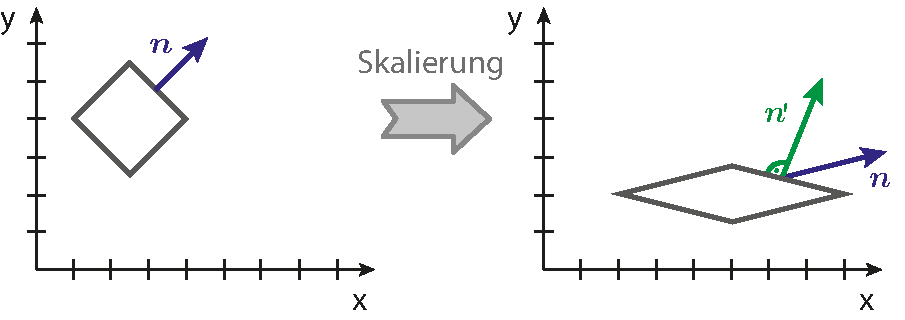
\includegraphics[width=1\textwidth]{./img/transformation/normale_skalierung.pdf}
    \caption{Die Raute und ihre Normale $\boldsymbol{n}$ werden auf die gleiche Art und Weise transformiert und zwar auf die doppelte Breite und halbe Höhe skaliert. Nach der Skalierung steht $\boldsymbol{n}$ nicht mehr orthogonal auf der Oberfläche. Die korrekte Normale ist $\boldsymbol{n'}$. D.h. die Normale muss bei der Transformation gesondert behandelt werden.
    }
    \label{fig:normale_skalierung}
\end{figure}

%Auch am Schnittpunkt eines transformierten Objekts wird eine Normale \( \vv{n'} \) benötigt.
Momentan ist der "`Raytracer"' in der Lage den Schnittpunkt eines Primärstrahls mit einem transformierten Objekt zu berechnen. Was fehlt, ist die Normale an diesem Schnittpunkt. Problematisch ist die Tatsache, dass die Normalen jeweils nur für die untransformierten Objekte erzeugt werden (s. Kapitel~\ref{ch:obj_schnitt}).
Abb.~\ref{fig:normale_skalierung} verdeutlicht, dass auf diese Normalen nicht einfach die gleiche Transformation angewendet werden kann, die für das Objekt verwendet wurde. Denn nach der Skalierung steht \( \boldsymbol{n} \) in der Abbildung nicht länger senkrecht auf der Oberfläche des Objekts. Die korrekte Normale ist \( \boldsymbol{n'} \). 

Nach \cite{pharrhumphrey2010Physically} (S. 87) ist es das Ziel, \( \boldsymbol{n} \) derart zu transformieren, dass dabei \( \boldsymbol{n'} \) herauskommt. 
Zur Veranschaulichung stellt man sich eine ebene Oberfläche vor, in der zwei Punkte liegen. Die Differenz der Punkte bildet einen Tangentialvektor. Nach einer Transformation liegen die Punkte weiterhin in der ebenen Oberfläche und somit auch der Tangentialvektor.
Das heißt, wird auf den Tangentialvektor einer Oberfläche die gleiche Transformation angewandt, wie auf die Oberfläche selbst, bleibt er weiterhin Tangentialvektor.

Nun bedient man sich der Tatsache, dass die Normale \( \boldsymbol{n} \) senkrecht auf dem Tangentialvektor \( \boldsymbol{t} \) steht und damit ihr Skalarprodukt Null ergibt. Nach der Transformation muss auch die neue Normale \( \boldsymbol{n'} \) senkrecht auf dem transformierten Tangentialvektor \( \boldsymbol{t'} \) stehen. Dabei ist \( \boldsymbol{T} \) die Transformation, die auf die Oberfläche und den Tangentialvektor angewendet wird, und \( \boldsymbol{S} \) ist die gesuchte Transformation, die auf die Normale anzuwenden ist.
Somit ist:

\begin{align*}  
    0 &=  \boldsymbol{t'} \cdot \boldsymbol{n'} \\
    0 &=  \left( \boldsymbol{S} \cdot \boldsymbol{n} \right) \cdot \left( \boldsymbol{T} \cdot \boldsymbol{t} \right) \\
    0 &= \left( \boldsymbol{S} \cdot \boldsymbol{n} \right)^\intercal \left( \boldsymbol{T} \cdot \boldsymbol{t} \right)  \qquad \qquad \text{siehe Gleichung \ref{eq:skalarprodukt}} \\
    0 &= \boldsymbol{n}^\intercal \left( \boldsymbol{S}^\intercal \cdot \boldsymbol{T} \cdot \boldsymbol{t} \right)
\end{align*}

Wie bereits erwähnt, gilt die Prämisse  \( \boldsymbol{n}^\intercal \boldsymbol{t} = 0 \), d.h. \( \boldsymbol{S}^\intercal \cdot \boldsymbol{T} \) muss letztendlich einfach aus der Gleichung verschwinden und somit die Einheitsmatrix ergeben. Damit \( \boldsymbol{S}^\intercal \cdot \boldsymbol{T} = \mathds{1} \) gilt, muss \( \boldsymbol{S}^\intercal = \boldsymbol{T}^{-1} \) sein.
Eine letzte Umformung liefert das Ergebnis \( \boldsymbol{S} = (\boldsymbol{T}^{-1})^\intercal \). Um eine Normale also korrekt zu transformieren, muss sie mit der transponierten Inversen der ursprünglichen Transformationsmatrix transformiert werden.




%0 &= \vv{t} \cdot \vv{n} \\
